% =============================================================================
% Victoria-Regia book template by @jancarauma
% 2025 (c) Janderson Gomes
% For further details, visit: artientista.blogspot.com (Caraumã)
% 16/06/2025 - amazon brazil
% =============================================================================

% Document class and layout settings
\documentclass[10pt,openany]{book}    % Standard book class with 12pt font and chapters starting on any page

% Golden ratio constant for layout calculations
\newcommand{\goldenratio}{1.618}

% Font encoding ensures proper glyph output
\usepackage[T1]{fontenc}

% for musical scores

\usepackage{musixtex} 

\usepackage{multicol}
\usepackage{wasysym} % for \longs
\usepackage{todonotes}

\def\nnotes{\vnotes1.6\elemskip}
\def\nnnotes{\vnotes1.28\elemskip}
\newcommand{\HRule}{\par
  \vspace*{\dimexpr-\parskip-\baselineskip+0pt}
  \noindent\rule{\linewidth}{0.5mm}\par
  \vspace*{\dimexpr-\parskip-.5\baselineskip+0pt}}
  
% --- Book metadata definitions ---
\newcommand{\authorname}{JaneAusten.cz}          % Primary author
\newcommand{\booktitle}{Tance JaneAusten.cz}     % Main title
\newcommand{\subtitle}{Primárně anglické kontratance období empíru}   % Subtitle (optional)
\newcommand{\publisher}{JaneAusten.cz}                 % Publisher name
\newcommand{\editionyear}{2025}                  % Edition year for print run


% Additional package imports (layout, styling, utilities)
\usepackage{misc/options}  % Custom configuration package (margins, headers)

\begin{document}

% ===== Front Matter =====
\frontmatter                      % Roman numerals for front matter
\pagestyle{empty}
% =================
% Title page
% =================
\begin{titlepage}
	\centering
	\newgeometry{top=1in,bottom=1in,right=0in,left=0in}
    \thispagestyle{empty}
	~	

    % Author name
	\vspace{24pt}
	{\scshape\large \authorname\par}

    % Book title
	\vspace{4pt}
	{\scshape\Huge \booktitle\par}

    % Subtitle (if defined)
    \ifx\subtitle\undefined\else
        \if\relax\detokenize\expandafter{\subtitle}\relax\else
            \vspace{6pt}
	        {\scshape\large \subtitle\par}
	        \vspace{\stretch{1.25}}
        \fi
    \fi

    % Translator (if defined)
    \ifx\translatorname\undefined\else
        \if\relax\detokenize\expandafter{\translatorname}\relax\else
            {\vspace{18pt}\itshape\large{Translated by}\par}
	        \vspace{6pt}
            {\itshape\Large\translatorname\par}
        \fi
    \fi

    % Publisher (bottom of the page)
    \vspace{\stretch{6}}
	{\Huge\scshape\large\publisher\par}
\end{titlepage}
     % Title page layout
% =================
% Copyright page
% =================
{\small
\setlength{\parindent}{0em}\setlength{\parskip}{1em}
~
\vfill

% First publication date
First edition, \editionyear{}

% Copyright notice
Copyright \copyright{} \editionyear{} Jindra Dítě

% License summary
% License summary
All content in this publication is licensed under the Creative Commons 
Attribution‑NonCommercial‑NoDerivatives 4.0 International License. You 
are permitted to share, copy, and redistribute the material in any 
medium or format, provided that proper credit is given to the original 
author, the content is not altered in any way, and the work is not used 
for commercial purposes. For full license terms, visit 
\url{http://creativecommons.org/licenses/by-nc-nd/4.0/}.

If you have any questions, please feel free to contact the author by \\ \textbf{example.com}.


% ISBN (if available)
\ifx\isbn\undefined\else\if\relax\detokenize\expandafter{\isbn}\relax\else{ISBN \isbn{}}\fi\fi

% Publisher logo
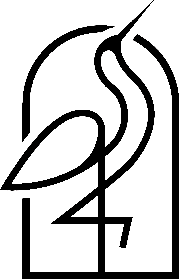
\includegraphics[width=0.07\linewidth]{frontmatter/logo-black.png}

% Publisher name
Published by \publisher{}
}
     % Copyright and licensing information
\usepackage{hyperref}% =================
% Preface page
% =================
\chapter{Úvodem}

\lettrine{P}{rávě v ruce držíte tuto knížečku}, či si ji snad prohlížíte na monitoru počítače. Pokud čtete tento text, netuším jak se vám dostala do rukou. Možná jste na ni náhodně narazili při procházení internetu, možná jste na ni dostali odkaz když vám ji někdo potřeboval na rychlo předat, možná ji někdo vytiskl na workshop kde neměl čas (či náladu) napsat k ní předmluvu vlastní. Jak přesně se to stalo je vlastně jedno; knížečka je vám plně k dispozici. Čtěte ji jak srdce touží, sdílejte ji bez obav, k tomu je určená. Chcete-li nejnovější verzi této knížečky, najdete ji na \url{https://github.com/Adrijaned/JaneAustenDances.LaTeX}, jenom prosím, ponechte někde v knížce tento odkaz i pro ostatní :) Každopádně vám přeji mnoho úspěchů s tancem a nechť zde naleznete čeho si žádáte.

\section*{English Country Dances - Regency Dances - Kontratance - CO TO VLASTNĚ JE?}

Klíčovým slovem pro tance nejen období Regency je "Playford", neboli \textit{The English Dancing Master: or, Plaine and Easie Rules for the Dancing of Country Dances, with the Tune to each Dance} (Anglický taneční mistr, aneb Prostá a jednoduchá pravidla tančení venkovských tanců, s melodií ke každému tanci), kterou v letech 1651-1728 vydal John Playford, jeho synové a následovníci. Tato sbírka byla téměř do konce 19. století hlavním zdrojem tanců pro jak venkovské, tak zámecké taneční večery a plesy. Později ji následovaly sbírky vydané dalšími autory či vydavateli. V dnešní době už také existují tance, které vytvořili soudobí tanečníci ECD na staré melodie a které doplňují a  zpestřují paletu těch původních.

Obecně se jedná o tance společenské, kde tanečníci často netancují pouze se svým partnerem, nýbrž i ostatními tanečníky okolo, to vše v prostorově zajímavých tancích sestávajících zpravidla z jednoduchých figur. Tančit lze obyčejným krokem, případně i kroky tanečními dle zdatnosti tanečníků. Velké oblibě se tyto tance těšily hlavně mezi střední třídou Anglie v 17. - 19. st., v určitých variacích jsou ale lokálně často tančené dodnes (hlavně v rámci USA).

\section*{A trocha reklamy...}

Pokud vás tento typ tanců zaujal a chtěli byste si někde zatančit naživo,
\begin{description}
    \item[V Brně] funguje spolek JaneAusten.cz, který pořádá \textbf{jednou měsíčně} neformální tančírny v Brně (3h blok výuky/tance otevřený i nováčkům), nepravidelně poté empírové plesy a různé další tematické akce. Více informací je k nalezení na stránkách www.janeausten.cz a na Facebooku.
    \item[V Praze] pořádá Páv Lučištník každé druhé pondělí Kontra-Po - kontratancové pondělky podobného formátu jako neformální tančírny v Brně, jednorázově poté i další akce. Více na https://oook.cz/
\end{description}

\cleardoublepage   % Make sure contents page starts on right-side page       % Preface or acknowledgments section
% =================
% Table of contents
% =================
\tableofcontents % Automatically generates the table of contents based on \section, \chapter, etc.

%\thispagestyle{empty} % Removes page number from this page (useful for clean presentation)
\cleardoublepage      % Ensures the next content starts on a right-hand (odd-numbered) page       % Table of contents

% ===== Main Content =====
\mainmatter                       % Switch to Arabic numbering
\pagestyle{fancy}                 % Fancy headers and footers for chapters

% Chapter inputs
\inputdance{content/all_in_a_garden_green}
\inputdance{content/emmas_waltz}
\inputdance{content/hole_in_the_wall}
\inputdance{content/indian_queen}
\inputdance{content/jamaica}
\inputdance{content/my_lord_byrons_maggot}
\inputdance{content/pauls_alley}
\inputdance{content/rakes_of_rochester}
\inputdance{content/row_well_ye_mariners}
\inputdance{content/swedish_country_dance}
\inputdance{content/upon_a_summers_day}

% ===== Back Matter =====
\backmatter                       % Unnumbered appendices and bibliography

\end{document}